\documentclass[]{sig-alternate}
\usepackage{graphicx}
\usepackage{epstopdf}
\usepackage{url}
\renewcommand{\topfraction}{0.85}
\renewcommand{\textfraction}{0.1}

\conferenceinfo{TBD}{TBD}
\CopyrightYear{2012}
\crdata{}

\begin{document}

\title{Tuning a Lustre File System for Wide Area Network Deployment}
\subtitle{A study of LNET behavior over high bandwidth, high latency networks}

\numberofauthors{5}
\author{
\alignauthor Scott Michael\\
	\affaddr{Indiana University}\\
	\affaddr{Bloomington, IN 47408}\\
	\email{scamicha@iu.edu}
\alignauthor Liang Zhen\\
        \affaddr{Whamcloud Inc.}\\
        \affaddr{BLAH}\\
        \email{BLAH}
\alignauthor Robert Henschel\\
        \affaddr{Indiana University}\\
        \affaddr{Bloomington, IN 47408}\\
        \email{henschel@iu.edu}
\and
\alignauthor Stephen Simms\\
	\affaddr{Indiana University}\\
	\affaddr{Bloomington, IN 47408}\\
	\email{ssimms@indiana.edu}
\alignauthor Eric Barton\\
        \affaddr{Whamcloud Inc.}\\
        \affaddr{BLAH}\\
        \email{BLAH}
\alignauthor Matthew Link\\
	\affaddr{Indiana University}\\
	\affaddr{Bloomington, IN 47408}\\
	\email{mrlink@indiana.edu}		
}

\maketitle

\begin{abstract}

\end{abstract}

\category{H.3.4}{Information Storage and Retrieval}{Systems and Software}[Distributed systems, Performance evaluation (efficiency and effectiveness)]
\category{C.2.2}{Computer-Communication Networks}{Network Protocols}[Protocol architecture (OSI model),
Routing protocols]

\terms{Algorithms, Performance}

\keywords{WAN file systems, Lustre, Data Superconductor}
\vspace{0.25in}
\section{Introduction}\label{sec:intro}


\section{Lustre and the LNET Protocol}\label{sec:LNET}

\subsection{RPCs in Flight}

\subsection{Peer Credits}
 

\section {An Example Case}\label{sec:usecase}


\section{System Setup}\label{sec:setup}
The systems used for testing are composed of three main parts, the compute resource, the network, and the data storage resource, which are described below for both the DC-WAN and MSU local Lustre setups.

\subsection{Compute Resource}



\subsection{Network}


\subsection{Lustre Hardware and Configuration}
\subsubsection{Hardware}\label{sec:hardware}

Figure \ref{fig:hardwaresetup} shows the final configuration that was used between Seattle and
Indianapolis. IBM provided 31 servers that functioned as compute nodes as well as the 16 storage servers that
were attached to the DataDirect Networks (DDN) storage devices. Brocade and Ciena provided the routing
equipment that enabled the network link from the show floor to Indianapolis.

The configurations of the compute cluster, storage, and networking components were identical in both Indianapolis and
Seattle. The core networking component at each endpoint was a Brocade MLXe-16 router that provided a 100 Gbps
Ethernet connection to the Ciena optical terminal managed by Internet2. The core router also provided a 10
Gbps link to an IBM BNT G8264 OpenFlow enabled switch at each endpoint. These switches were connected at 10 Gbps
over a separate Internet2 connection. The 31 compute servers and 16 Lustre storage
servers were attached directly to the Brocade core router at 10 Gbps using Twinax cables and Brocade 1860
dual-port adapters.

The compute servers were IBM System x iDataPlex dx360 M3 systems, each configured with dual Intel Xeon E5645
6-core 2.40 GHz processors, 24 GB of DDR3 RAM, a Brocade 1860 adapter, and a 250 GB SATA hard drive. The
object storage servers (OSS) were IBM System x iDataPlex dx360 M3 servers each configured with an Intel Xeon
E5645 6-core 2.40 GHz processor, 48 GB of DDR3 RAM, a Brocade 1860 adapter, and a 1 TB SATA hard drive. The
OSS nodes at each site were connected directly to a DDN SFA10000 via 8 Gb Fibre Channel (FC). The SFA10000
drove five 60-slot storage enclosures configured with 2 TB SATA disk drives. The metadata server was identical
to the compute servers, except it had 96 GB of RAM and was directly connected to a DDN EF3015 RAID system that
contained twelve 300 GB 15K RPM SAS disk drives for Lustre metadata.

Due to space constraints on the show floor server density was important. The dual-port Brocade 1860 adapters
were able to saturate the 8 Gb FC links as well as the 10 Gbps Ethernet links simultaneously, allowing the use
of rack dense IBM iDataPlex servers with only one PCI-Express slot available. The throughput of the DDN
SFA10000 allowed us to use a single storage system for the Lustre OSS nodes at each site.

\begin{figure*}
\begin{center}
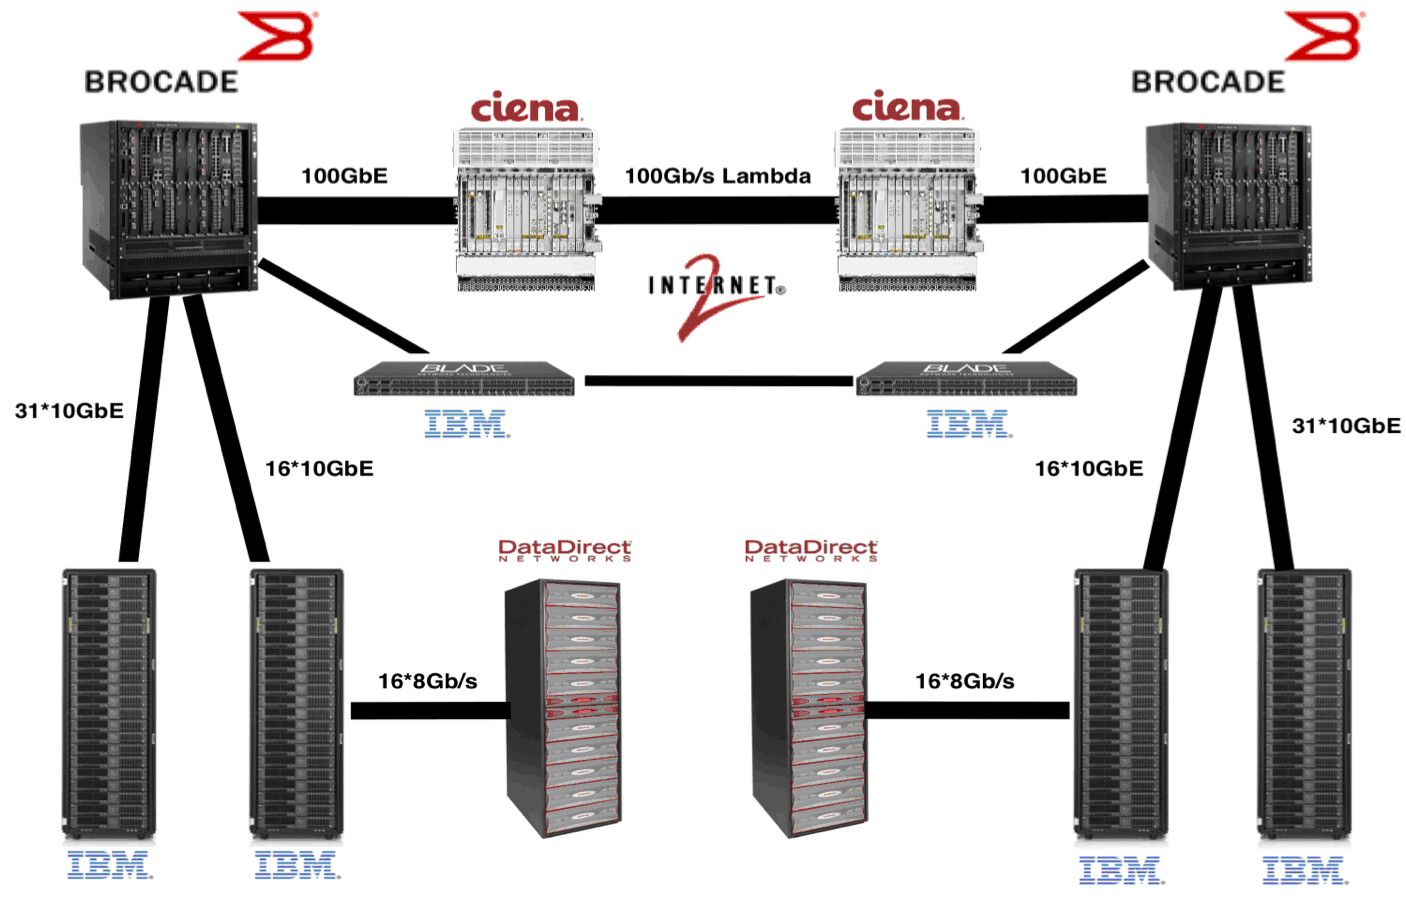
\includegraphics[width=0.80\textwidth]{figures/Figure1.png}
\caption{Hardware setup}
\label{fig:hardwaresetup}
\end{center}
\end{figure*}


\subsubsection{Software Configuration}




\section{Results}\label{sec:results}

\section{Discussion}\label{sec:discussion} 

\section{Conclusions}\label{sec:conclusions}
  

\section{Acknowledgments}

\bibliographystyle{abbrv}
\bibliography{general}
\end{document}
